\documentclass{article}
\usepackage[margin=0.8in]{geometry}
\usepackage{amsmath}
\usepackage{bookmark}
\usepackage{hyperref}
\usepackage{graphicx}
\usepackage{float}

\title{Mini-Assignment 2: CS3423 - Compilers - II}
\author{S Vishwak\\
\texttt{CS15BTECH11043}}
\date{}

\begin{document}
\maketitle

\section{Architecture and Design of Polly}
\begin{flushleft}
Polly is a tool used to optimize loops better than those achieved by the regular optimization tags such as \texttt{-O3} or \texttt{-O2}. It operates on the intermediate representation generated by LLVM. Below is a general representation of the compilation of a program using LLVM tools:
\begin{center}
\boxed{\text{Code}} \(\Rightarrow\) \boxed{\text{Tokens}} \(\Rightarrow\) \boxed{\text{AST}} \(\Rightarrow\) \boxed{\text{LLVM IR}} \(\Rightarrow\) \boxed{\text{Optimized LLVM IR}} \(\Rightarrow\) \boxed{\text{Binary}}
\end{center}

Since the focus of this assignment is the optimization w.r.t. Polly, the rest of this section will discuss about the placement and role of Polly in the penultimate step involving raw LLVM IR and the optimized LLVM IR.
\(\newline\)

According to \href{http://polly.llvm.org/docs/Architecture.html}{Polly's Architecture}, every optimization pass i.e., whenever you give the optimization flag (for example: \texttt{-O1}, \texttt{-O2}), there are a series of passes that take place one after the other, which all after completion render the optimized LLVM IR. These phases are broadly listed as follows:
\begin{itemize}
\item Canonicalization
\item Inliner-Cycle
\item Target Specialization
\end{itemize}

\underline{Canonicalization} tries to achieve maximum reduction/elimination of the raw IR using scalar optimizations, hence the name ``canonical". \underline{Inliner-Cycle} focuses on further scalar optimization without disrupting the semantic meaning of the code given and repeatedly tries to inline functions and runs canonicalization passes when the chance of simplification arises, making this a ``Soup algorithm"\footnote{Reference to Ramakrishna sir's notion of Soup algorithm} of sorts. One highlight of the \underline{Inliner-Cycle} is that, simple trivial loop optimizations are done - one such being LICM\footnote{Loop Invariant Code Motion}. Finally comes the \underline{Target Specialization}, which is exactly as it seems - takes into consideration the nature of the target such as the architecture. Some loop transformations occur here.
\(\newline\)

\subsection*{Where does Polly fit in?}
From the looks of it, you could add Polly in two places: 
\begin{itemize}
\item between \underline{Canonicalization} and \underline{Inliner-Cycle}, or
\item between \underline{Inliner-Cycle} and \underline{Target Specialization}
\end{itemize}

This positioning can be controlled using the option \texttt{-polly-position}. The tags taken by this option are: \texttt{early} and \texttt{before-vectorizer}. \texttt{early} indicates placing Polly in the first location suggested and \texttt{before-vectorizer} indicates placing Polly in the second location suggested. There is still some work being performed w.r.t. placing Polly in the second location, hence the default location is \texttt{-polly-position=early}.

\subsection*{How does the location matter?}
When placed in the first location, the optimized code generated by Polly is very similar to the raw LLVM IR. This leads to better understanding of the code produced and consequently better feedback. 
\(\newline\)

When placed in the second location, the Inliner-Cycle has been completed, which means there could be benefits theoretically from running Polly at this location. Since the loop kernel detection time is less, the compile time is not affected greatly. But since LLVM itself performs a whole lot of optimizations in the phases before reaching Polly, practically there could lesser effects than expected.

\subsection*{Capabilities of Polly}
\begin{itemize}
\item Extremely fast loop kernel detection
\item Performs loop optimization on functions which are ``worth" optimizing
\item Low compile time overheads
\end{itemize}
\end{flushleft}

\section{Some experiments with Polly}
\begin{flushleft}
Making some minor modifications to the \texttt{matmul.c}\footnote{Code taken from \texttt{https://github.com/llvm-mirror/polly/blob/master/www/experiments/matmul/matmul.c}} code provided as an example, I ran tests for varying N with 9 options:
\begin{enumerate}
\item Optimization with \texttt{-O3}
\item Optimization with Polly using \texttt{-mllvm -polly}
\item Optimization with Polly and parallelizing using \texttt{-mllvm -polly -mllvm -polly-parallel -llvm -polly-num-threads=i -lgomp} for \texttt{i} ranging from 1 to 4
\item Optimization with Polly using tiling \texttt{-mllvm -polly -mllvm -polly-tiling}
\item Optimization with Polly using vectorization \texttt{-mllvm -polly -mllvm -polly-vectorizer=stripmine}
\item Optimization using both tiling and vectorization
\end{enumerate}

Below are the compile time and run time results obtained:
\begin{figure}[H]
\begin{minipage}{0.45\linewidth}
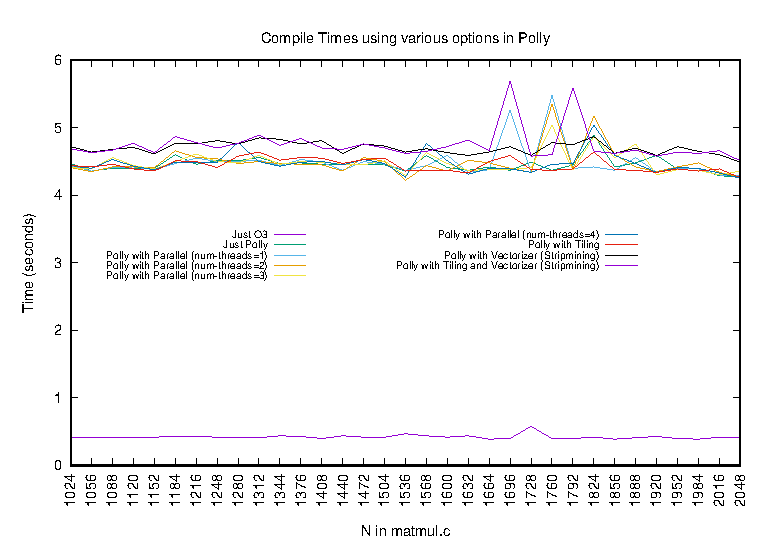
\includegraphics[width=0.9\textwidth]{./images/compile_time.eps}
\caption{Compile Time graph}
\end{minipage}
\hfill
\begin{minipage}{0.45\linewidth}
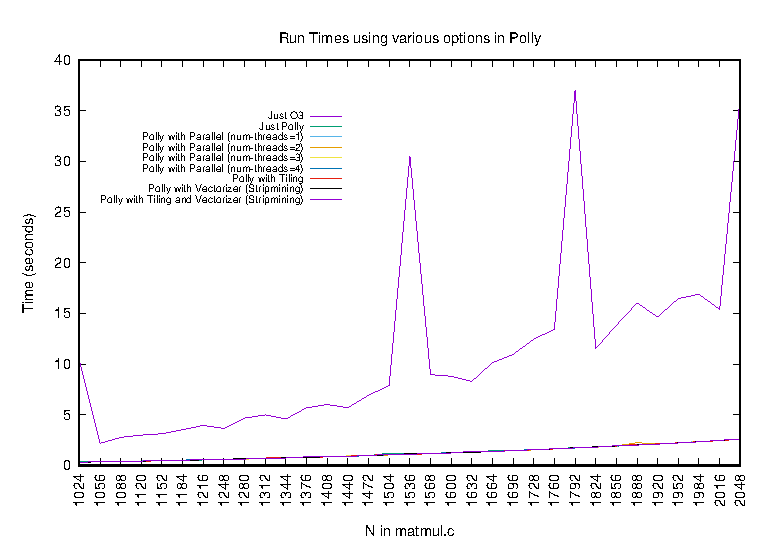
\includegraphics[width=0.9\textwidth]{./images/run_time.eps}
\caption{Run Time graph}
\end{minipage}
\end{figure}

Notice the amazing improvement in the run time over slight increase in compile for Polly based optimizations.
\end{flushleft}
\end{document}
